\section{Some Highlights }

\frame{\frametitle{Science Team}

\begin{itemize}
  \item Workshops and Reviews:
  \begin{itemize}
      \item LSST Science Platform Final Design Review, Tucson, AZ 12-14 April 2019.
      \item Community Broker Workshop, ls.st/cbw, Seattle, WA 19-21 June 2019.
  \end{itemize}
\item Liaisons with Science Collaborations:
  \begin{itemize}
   \item Continual presence at ``Stack Club'' to support LSST scientists and understand user needs.
   \item Science Team liaisons to science collaborations attend meetings, workshops and present DM status.
 \end{itemize}
\item Verification and Validation:
  \begin{itemize}
    \item LSST Data Management Acceptance Test Specification \citeds{LDM-639}.
    \item One new FTE working on DM verification since December 2018.
    \item Science verification workshop --- a collaboration between Comissioning,  DM and Camera Subsystems --- took place in June 2019.
 \end{itemize}

\end{itemize}
}

\frame{{Alert Production}

      \begin{itemize}
        \item{Proof-of-concept design for scalable Alert Filtering Service (formerly ``mini-broker''); see \citeds{DMTN-093}.}
      \end{itemize}

  \vspace{-0.3cm}
  \begin{center}
    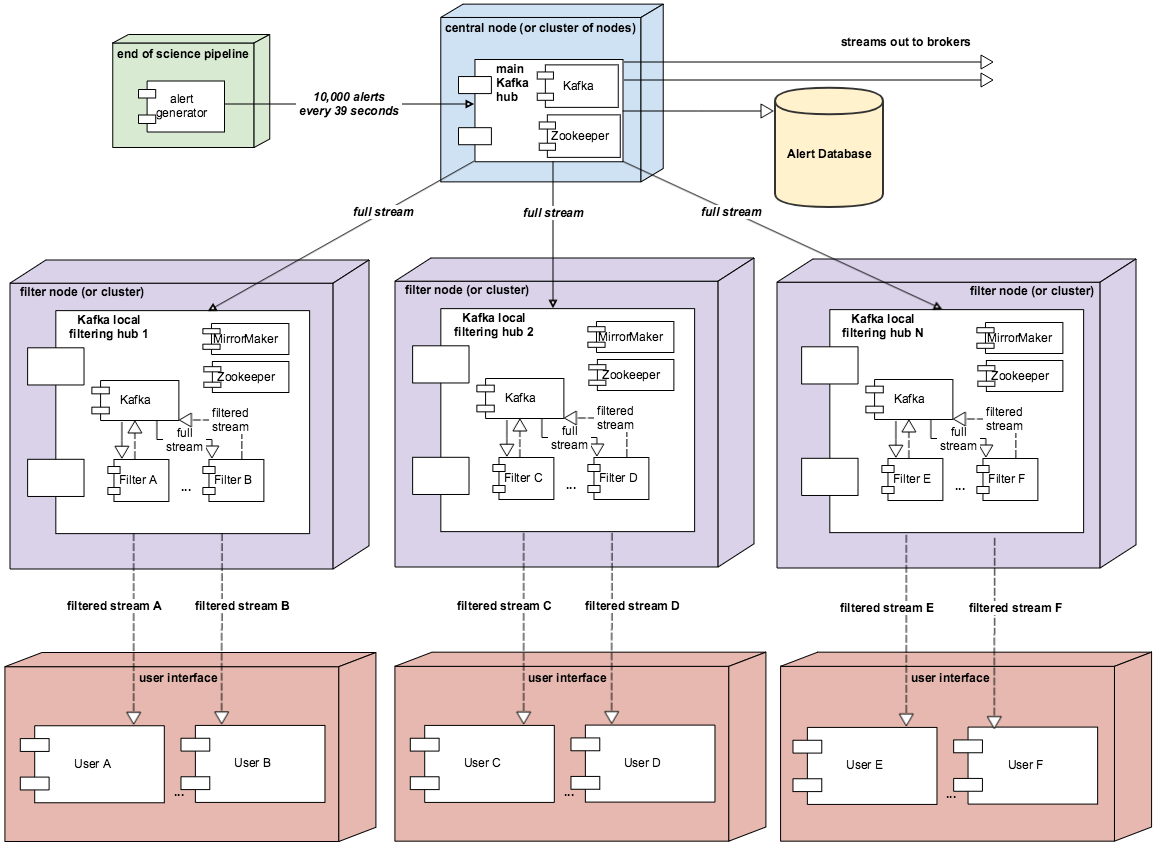
\includegraphics[width=0.5\textwidth]{figures/lafs.png}
  \end{center}
  \vspace{-0.7cm}
  \hspace{11.5cm}
  \tiny Figure: Patterson.

}

\frame{{Data Release Production}

  \begin{itemize}
   \item   {\textbf{LDM-503-07: Camera Data Processing}: Level 2 milestone demonstrating basic processing of data from \emph{physical LSST hardware} through Science Pipelines.}

        \item{The DRP team undertook a very successful ``sprint'' to integrate the SCARLET deblender \citep{2018A&C....24..129M} into the LSST Science Pipelines; it can now be run as part of regular LSST processing.}
            \item{The DRP team have integrated a version of the Forward Global Calibration Model \citep[FGCM;][]{2018AJ....155...41B} with the LSST Pipelines, and have extended it to provide absolute photometric calibration with respect to a reference catalog.}
 \item{A first protytpe of the one-dimensional spectral extraction pipeline designed to reduce data produced by the Auxiliary Telescope Spectrograph has been produced.}
           \item{Delivered partial mitigation for the brighter-fatter effect \citep{2014JInst...9C3048A}.}

  \end{itemize}

}

\frame{\frametitle{Base \& Network}
\begin{itemize}
\item Demonstrated 100\,Gbps from Base to NCSA in November at Supercomputing 2018.
\item 10\,TB of DECam data via SCInet via Miami -- Dallas -- Chicago.
\item Jupyter notebook used to monitor process from Data Transfer Node to disk at NCSA.
\end{itemize}
\centering
\vspace{-0.5cm}
\includegraphics[width=0.8\textwidth]{NetConfig2018}
}


\frame{\frametitle{Data Access Services}
\vspace{-0.2cm}

\begin{columns}
    \begin{column}{0.6\textwidth}
        \begin{itemize}
            \item Catalog Database (Qserv):
                \begin{itemize}
                   \item Currently hosting $\approx$ 175 TB across 30 nodes.
                     \begin{itemize}
                        \item NCSA: science dataset (Stripe 82 + WISE; Gaia DR2 soon).
                        \item CC-IN2P3: synthetic datasets.
                    \end{itemize}
                    \item Will scale to 75\% LSST DR1 by late 2019.
                    \item Cloud Deployment Demonstration \citedsp{DMTN-125}.
                    \begin{itemize}
                        \item Within 10-15\% perf. vs. dedicated hardware.
                    \end{itemize}
                \end{itemize}
            \item Web Services for Science Platform:
                \begin{itemize}
                    \item Built around IVOA standards.
                    \item TAP/ADQL query service (backed by Qserv) now online.
                    \item SODA image cutout service now online.
                    \item AstroPy PyVO Python client library improvements.
                \end{itemize}

        \end{itemize}
    \end{column}
    \begin{column}{0.4\textwidth}
        \begin{center}
            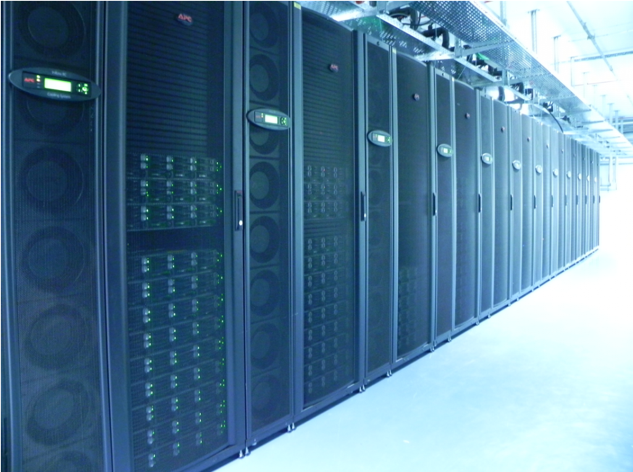
\includegraphics[width=\columnwidth]{figures/qserv-in2p3.png}
        \end{center}
    \end{column}
\end{columns}

}


\frame{\frametitle{LSST Data Facility (NCSA)}

\begin{itemize}
\item L2 Milestones completed: LDM-503-8b, LDM-503-8, LDM-503-4, LDM-503-4b.  % Would be good to say what these actually are!

\item Spectrograph integration tests, culminating in running prompt forwarder \& archiver processes on LATISS test stand in Tucson. Data is made available in ``Butler'' repositories at the Data Facility (caveat not optimal nor final).
\item Delivered multiple services: Kubernetes, Qserv, HTCondor. Plus authorization \& authentication support to LSST  in Chile.
\item Demonstrated Pegasus Workflow Management System (on HTCondor) and ``Butler'' based on an Oracle database running with ``Generation 3'' DM middleware. Since decided to go direct to HTCondor (dropping Pegasus).
\item Integrated of Camera Data Acquisition hardware on the L1 Test Stand at NCSA; provided a tutorial on the new software interface.
\item Led Operations Rehearsal \#1 to prepare for commissioning by simulating nominal operations during a three-day observation period.
\item Procured and configured test systems for ComCam; supplied to Tucson.

\end{itemize}
}

\frame{\frametitle{SQuaRE}

\begin{itemize}
  \item Notebook Aspect of the Science Platform now well established.
  \item New InfluxDB back-end for the SQuaSH (metrics curation) service.
  \item Also new: automated report creation from notebook templates.
  \item Prototyped DM Engineering \& Facility Database based on Kafka \& InfluxDB; demonstrated impressive scaling to 50\,Hz.

\end{itemize}
\begin{center}
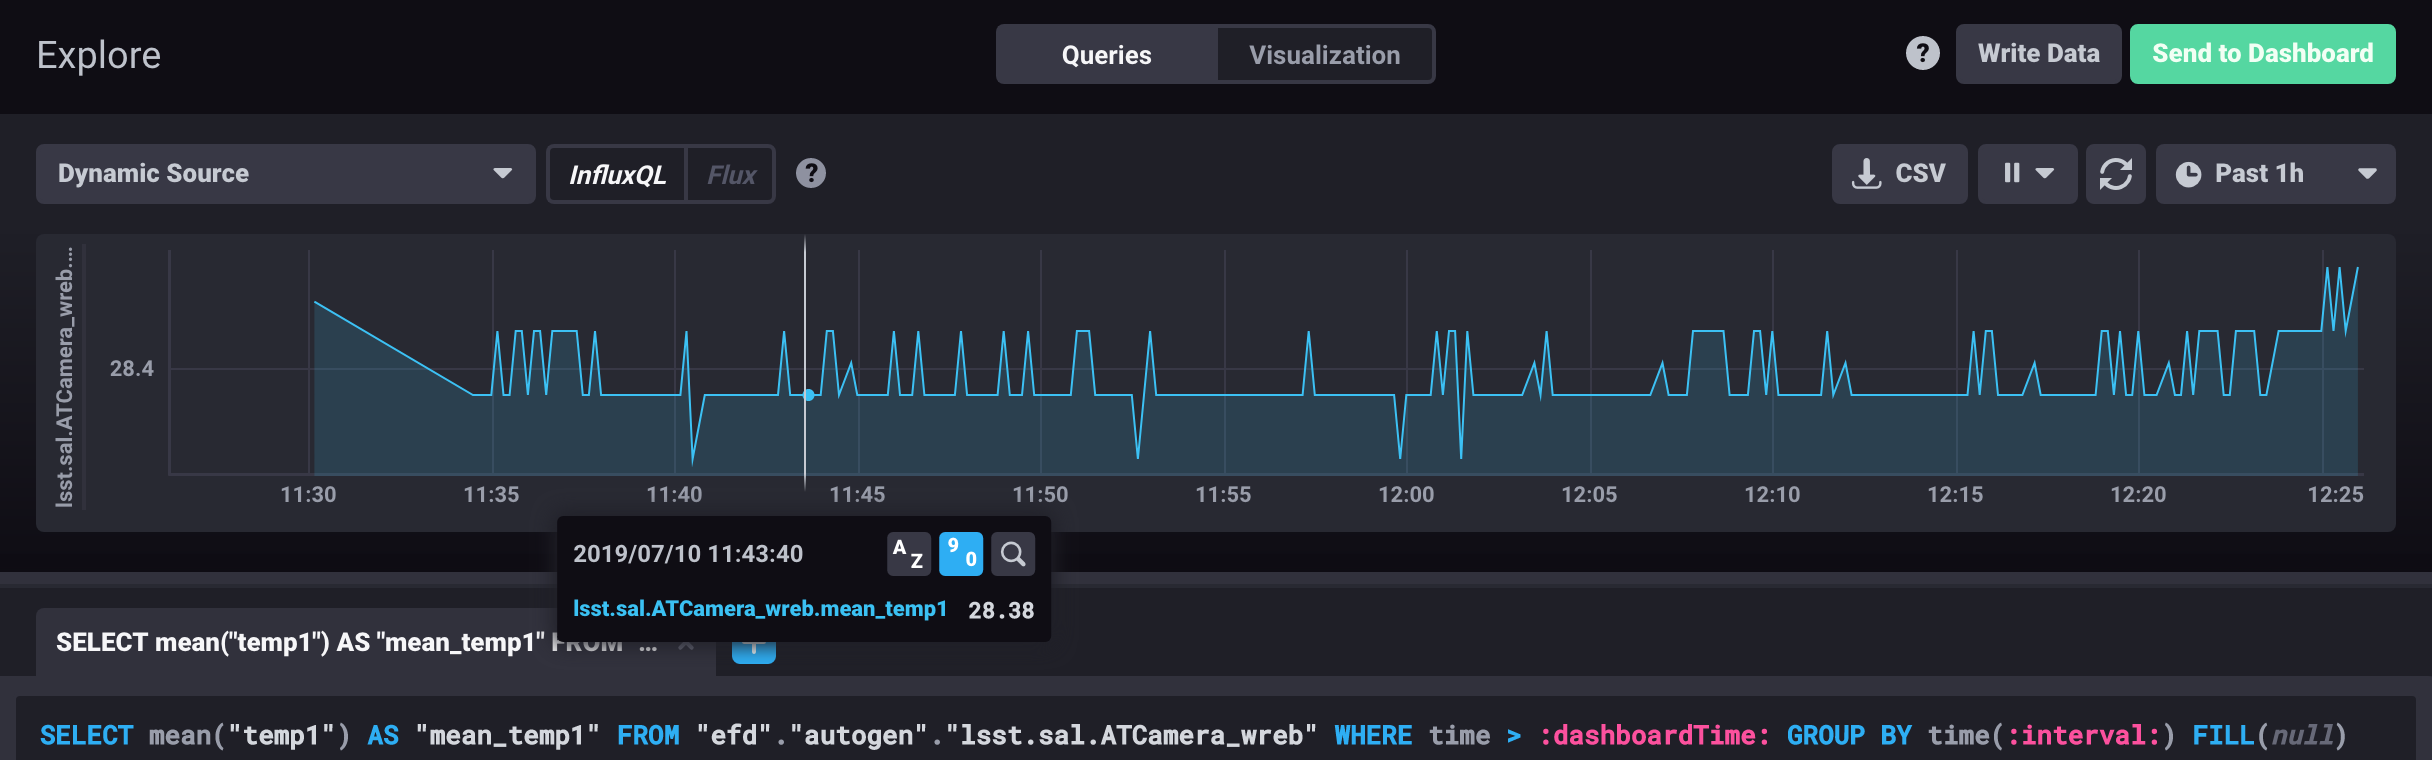
\includegraphics[width=0.8\textwidth]{figures/efd-live}
\end{center}
}

\frame{\frametitle{Milestone Burndown}
\begin{columns}
\begin{column}{0.45\textwidth}
\\
\includegraphics[width=1.1\textwidth]{images/burndownMiles}\\
\end{column}
\begin{column}{0.55\textwidth}
\begin{itemize}
\item All scheduled level 2 test milestones have been achieved since the last
review (some a little late)
\begin{itemize}
\item LDM-503-07    Camera Data Processing---\citeds{DMTR-112}
\item LDM-503-08    Spectrograph Data Acquisition---\citeds{DMTR-121}
\item LDM-503-08b   Small Scale CCOB Data Access---\citeds{DMTR-102}
\item LDM-503-09a   Science Pipelines Fall 2018 Release---\citeds{DMTR-111}
\item DMTC-8100-2112    Miami-Boca Raton path diverse fiber
\end{itemize}
\item We are carrying only 8 missed milestones (details in breakout)
\end{itemize}
\end{column}
\end{columns}
}

\frame {
  \frametitle{Hyper Suprime Cam (HSC) on Subaru}
        \vspace{-3mm}
        \begin{columns}
                \column{0.5\textwidth}
              \begin{center}
              \includegraphics[width=0.9\textwidth]{images/HSCcosmos}\\
              \end{center}
                      \column{0.5\textwidth}
                       \\
                       \vspace{1cm}
                       HSC image (COSMOS) from g, r (1.5 hrs), and i (3 hrs) bands; PSF matched co-add ($\approx 27.5$).\\
                       \vspace{3mm}
                       Processed with the \textit{LSST Science Pipelines}\\\url{https://pipelines.lsst.io/}.\\
                       \vspace{3mm}
                       We regularly reprocess data from HSC and other precursor facilities at the LSST Data Facility as part of our integration tests.\\
                       \vspace{10mm}
               {\tiny \bf{Image courtesy of the HSC collaboration \& Robert Lupton}}
               \end{columns}

}



\frame{\frametitle{ Reviews}
\begin{itemize}

\item{Just finished Joint Directors Review - 2 recommendations
  \begin{itemize}
    \item{ More cloud. }
    \item{ tooling for workflows especially debugging .}
	\item {General feed back was positive.}
  \end{itemize}
}
\item{Joint status review end of the month. }


\end{itemize}
}

